%%%%%%%%%%%%%%%%%%%%%%%%%%%%%%%%%%%%%%%%%%%%%%%%%%%%%%%%%%%%%%%%%%%%%
%%                                                                 %%
%% Please do not use \input{...} to include other tex files.       %%
%% Submit your LaTeX manuscript as one .tex document.              %%
%%                                                                 %%
%% All additional figures and files should be attached             %%
%% separately and not embedded in the \TeX\ document itself.       %%
%%                                                                 %%
%%%%%%%%%%%%%%%%%%%%%%%%%%%%%%%%%%%%%%%%%%%%%%%%%%%%%%%%%%%%%%%%%%%%%
\RequirePackage{tikz}

\documentclass[pdflatex,referee,iicol,sn-basic]{sn-jnl}

%%%% Standard Packages
\usepackage{xcolor,hyperref}
\usepackage[autostyle=false, style=english]{csquotes}
%%%%

% Avoid having to ``quote'' verbosely (csquotes package)
\MakeOuterQuote{"}

% Make Orcid icon
\definecolor{lime}{HTML}{A6CE39}
\DeclareRobustCommand{\orcidicon}{%
	
\begin{tikzpicture}
	\draw[lime, fill=lime] (0,0) 
	circle [radius=0.16] 
	node[white] {{\fontfamily{qag}\selectfont \tiny ID}};
	\draw[white, fill=white] (-0.0625,0.095) 
	circle [radius=0.007];
	\end{tikzpicture}
	\hspace{-2mm}
}

\foreach \x in {A, ..., Z}{%
	\expandafter\xdef\csname orcid\x\endcsname{\noexpand\href{https://orcid.org/\csname orcidauthor\x\endcsname}{\noexpand\orcidicon}}
}

% Define the ORCID iD command for each author separately.
\newcommand{\orcidauthorA}{0000-0002-3420-4576}
\newcommand{\orcidauthorB}{0000-0001-9402-0851}

%%%%%=============================================================================%%%%
%%%%  Remarks: This template is provided to aid authors with the preparation
%%%%  of original research articles intended for submission to journals published 
%%%%  by Springer Nature. The guidance has been prepared in partnership with 
%%%%  production teams to conform to Springer Nature technical requirements. 
%%%%  Editorial and presentation requirements differ among journal portfolios and 
%%%%  research disciplines. You may find sections in this template are irrelevant 
%%%%  to your work and are empowered to omit any such section if allowed by the 
%%%%  journal you intend to submit to. The submission guidelines and policies 
%%%%  of the journal take precedence. A detailed User Manual is available in the 
%%%%  template package for technical guidance.
%%%%%=============================================================================%%%%

\jyear{2021}%

%% as per the requirement new theorem styles can be included as shown below
\theoremstyle{thmstyleone}%
\newtheorem{theorem}{Theorem}%  meant for continuous numbers
%%\newtheorem{theorem}{Theorem}[section]% meant for sectionwise numbers
%% optional argument [theorem] produces theorem numbering sequence instead of independent numbers for Proposition
\newtheorem{proposition}[theorem]{Proposition}% 
%%\newtheorem{proposition}{Proposition}% to get separate numbers for theorem and proposition etc.

\theoremstyle{thmstyletwo}%
\newtheorem{example}{Example}%
\newtheorem{remark}{Remark}%

\theoremstyle{thmstylethree}%
\newtheorem{definition}{Definition}%

\raggedbottom
%%\unnumbered% uncomment this for unnumbered level heads

\begin{document}

\title[Synaptic and somatic short-term plasticity collaborate to yield deviance detection]{Short-term synaptic plasticity and threshold adaptation act in synergy to give rise to deviance detection in a spiking model of neuronal culture}

%%=============================================================%%
%% Prefix	-> \pfx{Dr}
%% GivenName	-> \fnm{Joergen W.}
%% Particle	-> \spfx{van der} -> surname prefix
%% FamilyName	-> \sur{Ploeg}
%% Suffix	-> \sfx{IV}
%% NatureName	-> \tanm{Poet Laureate} -> Title after name
%% Degrees	-> \dgr{MSc, PhD}
%% \author*[1,2]{\pfx{Dr} \fnm{Joergen W.} \spfx{van der} \sur{Ploeg} \sfx{IV} \tanm{Poet Laureate} 
%%                 \dgr{MSc, PhD}}\email{iauthor@gmail.com}
%%=============================================================%%

\author[1]{\fnm{Felix Benjamin} \sur{Kern} \orcidA{}}\email{kernfel@gmail.com}

\author*[1]{\fnm{Zenas C.} \sur{Chao} \orcidB{}}\email{zenas.c.chao@gmail.com}

\affil[1]{\orgdiv{International Research Center for Neurointelligence (WPI-IRCN)}, \orgname{The University of Tokyo}, \orgaddress{\city{Tokyo}, \country{Japan}}}

%%==================================%%
%% sample for unstructured abstract %%
%%==================================%%

\abstract{TODO}


\keywords{keyword1, Keyword2, Keyword3, Keyword4}

\maketitle

\section{Introduction}\label{sec-intro}


\section{Methods}\label{sec-methods}

\subsection{Model}\label{sec-model}

We modeled neurons as leaky integrate-and-fire units whose membrane potential $v$ at time $t$ followed
\begin{equation}
    \tau_m \frac{dv}{dt} = (v_{rest}-v) + I_{syn}(t)
\end{equation}
with $tau_m = 30$~ms the membrane time constant and $v_{rest} = -60$~mV the resting membrane potential. Synaptic currents were modeled in a conductance-based manner, following
\begin{equation}
    I_{syn} &= g_e(E_e-v) + g_i(E_i-v)
\end{equation}
with $E_e = 0$~mV and $E_i = -100$~mV the excitatory and inhibitory reversal potentials, respectively. Synaptic conductances evolved according to
\begin{align} 
    \tau_e \frac{dg_e}{dt} &= -g_e + \sum_{j \in \boldsymbol E} U x_j w \delta(t - \hat{t_j}) \nonumber \\
    \tau_i \frac{dg_i}{dt} &= -g_i + \sum_{j \in \boldsymbol I} w \delta(t - \hat{t_j}) \label{eqn-gsyn}
\end{align}
with $\tau_e = 2$~ms the excitatory time constant, echoing AMPA receptor dynamics \citep{Hausser1997-cn}, $\tau_i = 4$~ms the inhibitory time constant, echoing GABA-A receptor dynamics \citep{Destexhe1994-oc}, $\boldsymbol E$ and $\boldsymbol I$ the sets of presynaptic excitatory and inhibitory neurons, respectively, $w$ the synaptic weight, $\delta(\cdot)$ the Dirac delta function, and $\hat{t}$ the spike times.

Excitatory, but not inhibitory, synapses were subject to short-term depression (STD), simplified from \cite{Tsodyks1997-qt}; since synaptic transmission was not stochastic, we modeled the depression variable $x_j$ as a property of the presynaptic neuron $j$,
\begin{equation}
    \tau_x \frac{dx_j}{dt} = (1-x_j) - U x_j \delta(t - \hat{t}) \label{eqn-xsyn}
\end{equation}
with recovery time constant $\tau_x = 150$~ms and release fraction $U = 0.4$.

When a neuron's membrane potential reached the firing threshold $v_\theta$, a spike was emitted, and the potential was clamped to $v = v_{reset} = -74$~mV for a fixed refractory period of 3~ms (excitatory neurons). Inhibitory neurons were modeled as fast-spiking cells with a refractory period of 2~ms and a constant firing threshold $v_\theta = \theta_0 = -54$~mV \refp{Mensi2012-au}. In contrast, excitatory neurons were modeled with threshold adaptation (TA) as in \cite{Teeter2018-iz}, following
\begin{align}
    v_\theta &= \theta_0 + V_{TA}(t) \nonumber \\
    \tau_{\theta} \frac{dV_{TA}}{dt} &= -V_{TA} + \hat{\theta} \delta(t - \hat{t}) \label{eqn-TA}
\end{align}
with increment $\hat{\theta} = 1$~mV and decay time constant $\tau_{\theta} = 1$~s \refp{Pozzorini2015-ei}.

\begin{figure*}%
    \centering
    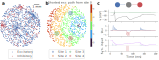
\includegraphics{fig1.pdf}
    \caption{}
    \label{fig1}
\end{figure*}
\textbf{Fig. 1}Model and paradigm. \textbf{a} Membrane and synaptic dynamics of a neuron innervated by an excitatory and an inhibitory neuron, illustrated above the plots, firing pre-determined spikes. The excitatory connection has weight $w = 3$ for demonstration purposes only; a single connection with $w = 1$ is normally unable to evoke postsynaptic firing. Top: Membrane voltage (black), firing threshold baseline (gray) and adaptive threshold (green) demonstrating TA. Middle: Excitatory ($g_e$, blue) and inhibitory ($g_i$, red) synaptic conductances, demonstrating excitatory STD. Bottom: Inputs to $g_e$ and $g_i$ (vertical bars in the appropriate colors), and the depression variable $x$ of the excitatory presynaptic neuron (dashed line). \textbf{b} Sample network layout, showing excitatory and inhibitory neurons and all outgoing synaptic connections from two neurons of each type. \textbf{c} Distance from stimulation site 0 in terms of minimum number of excitatory synapses. Stimulation is provided to the 10 neurons nearest to the center of each of 5 stimulation sites (round markers), which are regularly spaced on a circle with a radius of 2.5 mm.

Figure \ref{fig1}a shows the internal and presynaptic dynamics of an excitatory neuron in a contrived example for the purpose of illustration. The model was implemented in Brian2 \citep{Stimberg2019-tc}, accelerated with Brian2GeNN \citep{Stimberg2020-go}, and simulated with an integration time step of 1~ms. Synaptic delay was not modeled explicitly, but spikes were delivered, and voltages reset, in the time step following spike emission. We simulated neurons without any stochasticity in either their inputs or their parameters, other than network structure (described below), in order to ensure that our results were driven purely by the experimental paradigm, rather than any model-internal sources of noise.

800 excitatory and 200 inhibitory neurons were placed randomly in a two-dimensional circular space with a radius of 4~mm, and formed synapses of weight $w=1$ with 50 randomly selected postsynaptic partners within a range of 2~mm (excitatory) or 1~mm (inhibitory), reflecting the notion that excitatory neurons project over longer distances, while inhibitory neurons mainly connect to their local neighborhood. Connectivity and weights remained fixed throughout. Stimulation sites were evenly distributed 2.5~mm from the center of the dish, and stimulation delivered a one-time increase in $g_e$ to the 10 closest neurons, sufficient to trigger 2-3 spikes each. See Figure \ref{fig1}b and c for a representative example of the resulting network structure. Networks were pseudo-randomly generated according to the above scheme and screened for minimal stimulus response: Networks where fewer than 500 neurons responded to stimulation at any of the five sites after full recovery were discarded. In total, 30 networks were used for the experiments described below.

\subsection{Paradigm}\label{sec-paradigm}

To investigate deviance detection, we used a classical oddball paradigm as illustrated in Figure \ref{fig1}d, presenting a total of 500 stimuli at regular intervals of 500~ms. Target stimuli (labeled A hereafter) and distractor stimuli (labeled B to E) were presented in three randomized sequences: The "standard" sequence (std), consisting of 400 presentations of A and 100 presentations of B; the "deviant" sequence (dev) with 100 A and 400 B, and the many-standards control sequence (msc) with 100 presentations of each of the stimuli A through E. In this way, A is presented as the predominant and therefore expected stimulus (std), as an infrequent violation of an expectation (of B, dev), and, to control for pure adaptation effects, as an equally infrequent stimulus with no strong expectation of any particular input (msc).

In each network, we simulated oddball sequences with two A/B stimulus pairs (sites 1 and 2 in one pair, and sites 3 and 5 in the other pair), where each stimulus site in a pair was used once as target (A) and once as non-target (B), and a single msc sequence involving all sites. Networks were reset to a fully recovered state between sequence presentations to guarantee their independence. This yielded 4 complete data sets per network, or a total of 120 data sets across all networks.

In order to disentangle the effects of STD and TA, we ran all simulations in four conditions: Without any short-term plasticity, with either TA only or STD only, and with both STD and TA (labeled STD+TA in the following, and corresponding to the full model as described above). To turn off STD, we replaced Equation \ref{eqn-xsyn} with a constant $x = 1$, but retained the scaling of inputs to $g_e$ with $U$ in Equation \ref{eqn-gsyn}. This corresponds to immediate recovery ($\tau_x = 0$) and was done to maintain the magnitude of the excitatory postsynaptic potential (EPSP) in the recovered state regardless of whether STD was turned on or off. To turn off TA, we replaced Equation \ref{eqn-TA} with a constant $V_{TA} = 0$, making the firing threshold completely unadaptive.

\section{Results}\label{sec-results}

\subsection{Deviance detection}\label{sec-dd}

\begin{figure*}%
    \centering
    \includegraphics{fig2.pdf}
    \caption{}
    \label{fig2}
\end{figure*}
\textbf{Fig. 2} Deviance detection in vitro and in silico. \textbf{a} Response of a 2 \times 4~mm neuronal cell culture on a multi-electrode array, adapted from \cite{Kubota2021-dx}. Curves represent the average number of spikes per electrode in each 10~ms bin in response to target stimulation in the indicated sequence. Unlike in our study, oddball sequences here were split 10\%/90\%, and 10 equally frequent stimuli were used for the msc sequence. \textbf{b} Sample model response, showing average network-wide spike counts after stimulation with target (A) in the indicated sequence (same color code as panel \textbf{a}). Both in vitro and in the model, the dev response is very large, followed by an intermediate msc response and a low std response. \textbf{c} Mismatch, SSA and deviance detection indices (see Equation \ref{eqn-ddi}) across networks and stimuli (n = 120). In this and later boxplots, the median is indicated with an orange line, notches indicate the confidence interval for the median calculated by bootstrap with 10000 iterations, boxes indicate the inter-quartile range (IQR), whiskers extend to 1.5 times the IQR or to the data extrema, whichever is less, and fliers indicate individual data points beyond the whisker end points

We define deviance detection as a network's ability to pick out unexpected inputs from an otherwise homogeneous or otherwise unsurprising stream of inputs. Following related research \citep{Kubota2021-dx,Harms2014-ah,Jacobsen2001-sc}, we were careful to exclude effects due to stimulus identity (i.e., avoiding direct comparisons between different stimuli) or due to adaptation to frequent stimulus presentation (i.e., avoiding direct comparisons of A in the dev sequence to A in the std sequence). In other words, we used the msc sequence as a neutral baseline where the target stimulus was presented no more often than in the dev sequence, but no expectation of a competing stimulus B could be formed. To quantify deviance detection, we compared the mean number of spikes $R^A$ fired across the network in response to target stimulus A in the dev and msc sequences, defining a deviance detection index (DDI) as
\begin{equation}
    DDI = \frac{R^A_{dev} - R^A_{msc}}{R^A_{dev} + R^A_{msc}} \label{eqn-ddi}
\end{equation}
We define stimulus-specific adaptation (SSA, $R^A_{msc} - R^A_{std}$) and mismatch ($R^A_{dev} - R^A_{std}$) indices analogously, capturing respectively the effect of adaptation, and of both adaptation and deviance detection together.

Our first aim was to replicate deviance detection properties reported in dissociated neuronal cell culture by \cite{Kubota2021-dx}, reproduced in Figure \ref{fig2}a. In their case, cell cultures -- like our model, randomly connected networks with two-dimensional extent -- were stimulated at 10 different sites in msc sequences, and at two sites with 10\%/90\% probability in dev and std sequences. Deviance detection was assessed analogously to our definition of DDI and reached an average level of around 0.3 across two cultures.

In our model, we could readily identify networks and stimuli whose responses developed in a qualitatively similar fashion, with high activity in response to target in the dev sequence, low activity in the std sequence, and intermediate activity in the msc sequence, as illustrated with an example in Figure \ref{fig2}b. The model responses developed on a compressed time scale compared to neuronal culture, which we tentatively attribute to unfaithful aspects of the model, including a lack of conduction delay or spontaneous activity, a much smaller number of participating neurons, and structural differences.

Across networks and stimuli (Figure \ref{fig2}c), we found that our model reliably produced mismatch responses (t = 11.3, p = 6.7e-21; one-sided t-test for mismatch index > 0, n = 120) while both SSA index (t = 7.84, p = 1.05e-12) and DDI (t = 6.49, p = 1.05e-09) were also positive. The average DDI value reached around 0.1, which was less than the values reported by \cite{Kubota2021-dx}, but note that our target stimuli were presented more frequently (20\%) than theirs (10\%) in the dev and msc sequences.

\begin{figure*}%
    \centering
    \includegraphics{fig3.pdf}
    \caption{}
    \label{fig3}
\end{figure*}
\textbf{Fig. 3} Deviance detection under model ablation. \textbf{a} Sample network responses to target stimulation, with the deviance detection index in each instance noted in the plot titles. The color code is the same as in Figure \ref{fig2}. \textbf{b} SSA indices across all networks and stimuli. Asterisks indicate data greater than 0 at a significance level of p<0.05, see main text for detailed statistics. \textbf{c} Deviance detection indices across all networks and stimuli.

Having confirmed the presence of deviance detection in our model, we then turned to an ablation approach to try to identify how the two short-term plasticity mechanisms in the model, STD and TA, enabled the networks to learn relevant regularities. Figure \ref{fig3}a shows the responses to target stimulation of a sample network under ablation. With no plasticity, the responses are indistinguishable between sequences, yielding a DDI of 0, and indicating that stimulation did not have any long-lasting effects in membrane voltage or synaptic conductance. With STD only, the response in the dev sequence developed earlier and very slightly larger, yielding a DDI of 0.03. With TA only, the response became noticeably smaller, but the sequences became readily distinguishable, with high dev, intermediate msc, and low std responses, yielding a DDI of 0.19. Finally, in the full model, the dev response stood out more clearly, leaving much smaller msc and std responses and yielding a DDI of 0.4.

The SSA index (Figure \ref{fig3}b) was exactly 0 as expected in the ablation with no plasticity, and positive with any plasticity applied (STD only: t = 3.17, p = 0.000983, median 0.0039; TA only: t = 6.74, p = 3e-10, median 0.097; STD+TA: t = 7.84, p = 1.05e-12, median 0.135; one-sided t-tests, n = 120). Since the SSA index measures the degree of adaptation to frequent stimulus presentation, this indicates that both plasticity mechanisms were capable of imbuing the networks with some level of history dependence.

Finally, across networks and stimuli, the DDI (Figure \ref{fig3}c) was exactly 0 with no plasticity, not significantly different from 0 with STD only (t = -1.89, p = 0.0609, median -2.1e-04; two-sided t-test, n = 120), but clearly positive for TA only (t = 5.52, p = 1.01e-07, median 0.077; one-sided t-test, n = 120) and the full model (t = 6.49, p = 1.05e-09, median 0.114). To our surprise, the DDI of the full model was significantly greater than that of either plasticity mechanism alone (STD: t = 6.7, p = 4.53e-10; TA: t = 3.2, p = 0.00103), and greater too than the sum of the DDI values across both STD only and TA only models (t = 3.6, p = 0.000199). This suggests that TA and STD act not as independent mechanisms in this paradigm, but rather interact constructively to enhance the network's ability to encode input regularities.

In the following, we will use a sample network and target stimulus to first build an understanding of how TA leads to deviance detection when acting alone, i.e. in the ablated TA only model. Then, we will build on this understanding to elucidate how the addition of STD, which was shown above to be ineffective for deviance detection on its own, can lead to an increased deviant response in the full model.

\subsection{The role of TA in deviance detection}\label{sec-ta}

To understand why the same stimulus A evoked a higher response in dev than in msc, we first compared the average responses in the two conditions. As shown in Figure \ref{fig4}a, we found that the response developed in a qualitatively similar fashion, with a tendency of dev spikes to occur earlier, particularly shortly after stimulation, and more frequently, particularly towards the later part of the response. Since the stimulus was identical in both conditions, this difference had to be due to either changed firing thresholds, or changed synaptic currents as a consequence of activity differences in earlier parts of the response. We quantified the former with the strength of adaptation $V_{TA}$ (Figure \ref{fig4}b), which showed a clear and widespread lowering of thresholds at the start of dev trials relative to msc, followed by an increase beyond the msc baseline in many neurons as they spiked. Correlating the difference in $V_{TA}$ at the beginning of trials with the difference in trial spike count, we found that, across neurons, lower thresholds are strongly predictive of higher activity (r = -0.424, p = 3.1e-36, see Figure \ref{fig4}d).

To quantify the synaptic contributions to a neuron's membrane potential $v$, we calculated a quantity $V_{syn}$, shown in Figure \ref{fig4}c, which captures all synaptic inputs, but excludes voltage deflections caused by direct stimulation and by the self-inhibition induced by resetting to $v_{reset} < v_{rest}$ after a spike. Being induced by spiking activity, this measure closely followed the activity pattern, making the earlier activation of the dev response clearly visible across the network. In addition, since $V_{syn}$ decays with the membrane timescale $\tau_m$, but resets to $0$ on postsynaptic spikes, many of the neurons that spiked more frequently showed lower $V_{syn}$ towards the end of network activity.

\begin{figure*}%
    \centering
    \includegraphics{fig4.pdf}
    \caption{Responses and threshold adaptation in a TA-only ablation. \textbf{a, b, c} Post-stimulus histograms across target trials, showing trial time along the horizontal axis, and neurons along the vertical, sorted by the time of the first recorded spike across all trials and conditions. Left and middle column, target trials in dev and msc sequence, respectively; right column, contrast between these two. \textbf{d} Per-neuron relationship between the contrast (dev - msc) in $V_{TA}$ at the start of trials, and the contrast in average number of spikes fired, excluding inhibitory neurons, and associated linear regression (r = -0.424, p = 3.1e-36). \textbf{e} Contribution of $V_{TA}$ and $V_{syn}$ to bins with increased firing in dev (i.e., red bins in the spike probability contrast, \textbf{a}), weighted by that same contrast. \textbf{f} Contribution of $V_{TA}$ relative to the sum of the weighted contributions in \textbf{e}. \textbf{g} Relative contribution of $V_{TA}$ across networks, showing median (solid line) and inter-quartile range (shaded area)}
    \label{fig4}
\end{figure*}

\textbf{Fig. 4} Responses and threshold adaptation in a TA-only ablation. \textbf{a, b, c} Post-stimulus histograms across target trials, showing trial time along the horizontal axis, and neurons along the vertical, sorted by the time of the first recorded spike across all trials and conditions. Left and middle column, target trials in dev and msc sequence, respectively; right column, contrast between these two. \textbf{d} Per-neuron relationship between the contrast (dev - msc) in $V_{TA}$ at the start of trials, and the contrast in average number of spikes fired, excluding inhibitory neurons, and associated linear regression (r = -0.424, p = 3.1e-36). \textbf{e} Contribution of $V_{TA}$ and $V_{syn}$ to bins with increased firing in dev (i.e., red bins in the spike probability contrast, \textbf{a}), weighted by that same contrast. \textbf{f} Contribution of $V_{TA}$ relative to the sum of the weighted contributions in \textbf{e}. \textbf{g} Relative contribution of $V_{TA}$ across networks, showing median (solid line) and inter-quartile range (shaded area)

Based on these measures, we then asked why there were more spikes in dev trials. To answer this, we weighted the contrasts in $V_{TA}$ and $V_{syn}$ by the spike probability contrast, discarding any instances of equal or lower firing in dev, and summed over neurons. The resulting time courses (Figure \ref{fig4}e) reveal the immediate underlying causes of network-wide activity increases, namely de-adaptation and depolarization. We found that increased depolarization induced by synaptic input greatly outweighed the impact of reduced adaptation throughout most of the response. Only in the very early stages of the response did adaptation dominate the increase in firing (Figure \ref{fig4}f), whereas the late response was enlarged primarily as a result of increased presynaptic excitation. This trend was reflected in most networks investigated, as shown in the summary plot in Figure \ref{fig4}g. To summarize, while most added spikes arose from increased prior activity within a trial, the initial impetus -- the increase in the early response -- was largely caused by lower TA.

Having established that the increased response to A in dev trials was driven by lower thresholds, we next turned to the cause of this reduction. Firstly, plotting $V_{TA}$ at the start of A trials in Figure \ref{fig5}a, we found that most of the network was indeed less adapted in dev, with only a few neurons in the vicinity of B showing higher thresholds. We hypothesized that this could be due to the different non-target stimulation pattern, since B was stimulated more frequently in dev than msc. Indeed, as shown in Figure \ref{fig5}b, the non-target response activity in the dev sequence -- in other words, the response to B -- was concentrated around the site where B was delivered, while in the msc sequence, activity in response to the various non-target stimuli was dispersed across most of the network. Notably, although the comparison is between 400 B trials in dev, and only 100 B trials (alongside 300 C, D and E trials) in msc, only a small handful of neurons responded more to non-target stimulation in dev, most of these very close to the stimulation site of B.

\begin{figure*}%
    \centering
    \includegraphics{fig5.pdf}
    \caption{\textbf{a} $V_{TA}$ at the start of A trials (mean over trials), with each neuron shown in its spatial location. Left and middle column, raw averages for dev and msc sequences, respectively; right column, contrast between dev and msc averages. A and B stimulus locations for this and following figures are highlighted in the left plot; see Figure \ref{fig1} for the locations of the remaining stimuli used in the msc sequence. \textbf{b} Average response (in spikes per trial) to non-target trials (B in dev, B/C/D/E in msc). \textbf{c} Left and middle: Replacement and adaptation components of the non-target response contrast (\textbf{b}, right column), where replacement is the contrast (B msc - C/D/E msc), and adaptation is the contrast (B dev - B msc). Right: Network-wide mean replacement and adaptation values across networks and target stimuli. The adaptation effect is less than zero (t = -9, p = 2.02e-15), and less than the replacement effect (t = 2.3, p = 0.0119), which is not different from zero (t = -0.69, p = 0.246). \textbf{d} Per-neuron relationship between the contrast (dev - msc) in average number of spikes fired in response to non-target stimulation, and the contrast in $V_{TA}$ at the start of target trials, excluding inhibitory neurons, and associated linear regression (r = 0.99, p = 0). \textbf{e} The same relationship as \textbf{d}, but using the medians across excitatory neurons, and plotting one point per network and target stimulus. The values are highly correlated (r = 0.956, p = 5.98e-65)}
    \label{fig5}
\end{figure*}

\textbf{Fig. 5 a} $V_{TA}$ at the start of A trials (mean over trials), with each neuron shown in its spatial location. Left and middle column, raw averages for dev and msc sequences, respectively; right column, contrast between dev and msc averages. A and B stimulus locations for this and following figures are highlighted in the left plot; see Figure \ref{fig1} for the locations of the remaining stimuli used in the msc sequence. \textbf{b} Average response (in spikes per trial) to non-target trials (B in dev, B/C/D/E in msc). \textbf{c} Left and middle: Replacement and adaptation components of the non-target response contrast (\textbf{b}, right column), where replacement is the contrast (B msc - C/D/E msc), and adaptation is the contrast (B dev - B msc). Right: Network-wide mean replacement and adaptation values across networks and target stimuli. The adaptation effect is less than zero (t = -9, p = 2.02e-15), and less than the replacement effect (t = 2.3, p = 0.0119), which is not different from zero (t = -0.69, p = 0.246). \textbf{d} Per-neuron relationship between the contrast (dev - msc) in average number of spikes fired in response to non-target stimulation, and the contrast in $V_{TA}$ at the start of target trials, excluding inhibitory neurons, and associated linear regression (r = 0.99, p = 0). \textbf{e} The same relationship as \textbf{d}, but using the medians across excitatory neurons, and plotting one point per network and target stimulus. The values are highly correlated (r = 0.956, p = 5.98e-65)

We quantified the correlation between the differences in non-target response magnitude and strength of adaptation before target trials across excitatory neurons, and found an almost perfect relationship (Pearson's r = 0.99, n = 800, see Figure \ref{fig5}d). This effect was robust across networks: Greater reduction in the non-target response was closely correlated with a greater reduction in $V_{TA}$ at the start of A trials.

Finally, we examined the cause of the reduced response in non-target trials. Going from the msc sequence to the dev sequence, two things change: Firstly, stimulations with non-target C, D and E are replaced with B, which would cause different responses even in the absence of adaptation, and secondly, the more frequent presentation of B changes adaptation, reducing the average response. To estimate the effect of stimulus replacement and adaptation, respectively, we contrasted the response to B in the msc sequence with the response to other non-target stimuli in the same sequence (replacement), and with the response to B in dev (adaptation). We found that, in this particular network and stimulus pair, adaptation weakly but consistently decreased the response, whereas stimulus replacement reduced many responses more dramatically while permitting larger responses in many neurons in the general vicinity of the stimulus sites of A and B. Across networks, however, the effect of adaptation was more pronounced and more consistent, removing an average of 71 spikes per trial, whereas stimulus replacement had no effect on average.

To conclude, TA plays two complementary roles in deviance detection, affecting the standard and deviant response separately: On the one hand, it reduces the response to the frequently presented standard stimulus, leading to a larger deviant response merely by contrast with the corresponding standard (SSA). On the other hand, due to the overlap in receptive fields, TA acts as blanket suppression in the many-standards control condition, against which the deviant response, relieved from this suppression and encountering a less fatigued network, stands out.

\subsection{The role of STD in deviance detection}\label{sec-std}

As noted above, short-term depression alone exerted no deviance detection effect, but its addition did enhance the deviance detection effect established by TA. To understand the basis of this apparent synergy, we contrasted the TA-only condition examined in the previous section against the same network with both TA and STD. As shown in Figure \ref{fig6}, we found that the non-target response magnitude was reduced by the introduction of STD, as we would expect. Indeed, across networks, the response to all stimuli was reduced, regardless of context. Concomitantly, and in keeping with the above analysis, the levels of $V_{TA}$ before A trials also dropped.

\begin{figure*}%
    \centering
    \includegraphics{fig6.pdf}
    \caption{Contrast between the ablated model with only TA (shown in Figure \ref{fig5}) and the full model with both STD and TA. \textbf{a}, \textbf{b} Data shown in Figure \ref{fig5}ab, dev and msc columns, subtracted from the corresponding data for the full model. \textbf{c} Equivalent contrast (full - ablated model) in the response to A, in columns as above. \textbf{d} Network-wide mean $V_{TA}$ before A trials across networks. Left: Ablated and full model averages. Right: Difference between these model conditions. With the introduction of STD, $V_{TA}$ decreased more in dev than in msc (t = -3.49, p = 0.000342). \textbf{e} Mean number of spikes per target trial across networks. Left: Ablated and full model averages. Right: Difference between these model conditions. With the introduction of STD, the response decreased more in the std sequence than msc (t = -1.9, p = 0.0297), and more in msc than in dev (t = -2.99, p = 0.00168)}
    \label{fig6}
\end{figure*}

\textbf{Fig. 6} Contrast between the ablated model with only TA (shown in Figure \ref{fig5}) and the full model with both STD and TA. \textbf{a}, \textbf{b} Data shown in Figure \ref{fig5}ab, dev and msc columns, subtracted from the corresponding data for the full model. \textbf{c} Equivalent contrast (full - ablated model) in the response to A, in columns as above. \textbf{d} Network-wide mean $V_{TA}$ before A trials across networks. Left: Ablated and full model averages. Right: Difference between these model conditions. With the introduction of STD, $V_{TA}$ decreased more in dev than in msc (t = -3.49, p = 0.000342). \textbf{e} Mean number of spikes per target trial across networks. Left: Ablated and full model averages. Right: Difference between these model conditions. With the introduction of STD, the response decreased more in the std sequence than msc (t = -1.9, p = 0.0297), and more in msc than in dev (t = -2.99, p = 0.00168)

However, we noticed a systematic difference in the reduction of both response magnitude and $V_{TA}$ between the dev and msc conditions: The non-target response in the dev sequence was reduced more than that in the msc sequence, leading to a larger difference between the responses in these two contexts. $V_{TA}$ before A trials followed suit, leading to stronger de-adaptation and, as a consequence, a larger A trial response in dev in large parts of the network in the full model compared to TA-only. Across networks, only few cases of an increased dev response were seen; however, the response to the target stimulus (Figure \ref{fig6}e) was reduced least in dev, and most in std. This differential reduction was directly responsible for the larger DDI reported in Figure \ref{fig3}, but how did it arise?

Due to its relatively short time scale, the direct effect of STD across trials was likely limited to repeated trials of the same stimulus, such as the frequent stimulus in oddball sequences. However, by reducing the standard (i.e., the dev non-target) response in the full model, we hypothesized that STD also affects adaptation levels, causing de-adaptation and thereby indirectly increasing the target dev response.

In direct support of the notion that STD indeed carried over between (repeated) trials, we noted first that the response size in the STD-only condition was slightly less in std than in msc or dev (cf. Figure \ref{fig3}c), indicating some amount of SSA. To show that the across-trial effect of STD in the full model was limited to the dev non-target trials, however, we needed a more sophisticated tool, showing the level of depression experienced by each neuron. Since the effect of STD is to reduce excitatory postsynaptic potentials (EPSP), we estimated this reduction per synapse in a given trial type $S$ (e.g. A dev) as the product of the expected number of transmitted spikes $R^S$, the peak EPSP of the synapse ($k = 1.4 mV$, recall that all weights are 1), and its average depression coefficient $(1-x)$ at the start of the trial. Summing these estimates onto each postsynaptic neuron, we arrived at a rough estimate

\begin{equation}
    D^S = \sum_{i \in pre} R^S_i k (1-x_i^{t=0})
\end{equation}

of the average depolarization lost due to STD.

\begin{figure*}%
    \centering
    \includegraphics{fig7.pdf}
    \caption{\textbf{a} Estimated average STD-derived postsynaptic depression $D$ in target (A) trials (top row) and B trials (bottom row). Note that the difference between A and B in msc (middle column) is due only to the network configuration. \textbf{b} Statistics across networks of the contrast (dev - msc) in $D$ (cf. \textbf{a}, right column), and in $V_{TA}$ at the start of A trials (cf. Figure \ref{fig6}d). In each network, averages were taken over neurons with at least 0.2 spikes per dev trial (B trials for $\Delta D^B$, A trials for $\Delta D^A$ and $\Delta V_{TA}$). Whereas the third box ($\Delta V_{TA}$ total) indicates the averages in the full model, the final box ($\Delta V_{TA}$ added) indicates the difference between the full and the ablated (TA-only) model. This additional amount of $\Delta V_{TA}$, caused indirectly by the addition of STD, was less (i.e., more negative) than the directly STD-related $\Delta D^A$ itself (t = -2.09, p = 0.0195)}
    \label{fig7}
\end{figure*}

\textbf{Fig. 7 a} Estimated average STD-derived postsynaptic depression $D$ in target (A) trials (top row) and B trials (bottom row). Note that the difference between A and B in msc (middle column) is due only to the network configuration. \textbf{b} Statistics across networks of the contrast (dev - msc) in $D$ (cf. \textbf{a}, right column), and in $V_{TA}$ at the start of A trials (cf. Figure \ref{fig6}d). In each network, averages were taken over neurons with at least 0.2 spikes per dev trial (B trials for $\Delta D^B$, A trials for $\Delta D^A$ and $\Delta V_{TA}$). Whereas the third box ($\Delta V_{TA}$ total) indicates the averages in the full model, the final box ($\Delta V_{TA}$ added) indicates the difference between the full and the ablated (TA-only) model. This additional amount of $\Delta V_{TA}$, caused indirectly by the addition of STD, was less (i.e., more negative) than the directly STD-related $\Delta D^A$ itself (t = -2.09, p = 0.0195)

In Figure \ref{fig7}, we show that, in A dev and A msc trials, depression had relatively evenly distributed effects across the network. Neither sequence seemed to have a stronger overall effect, despite a slight trend towards weaker depression near the stimulus site in the dev sequence. In sharp contrast, in B dev trials, depression was very strong and very clearly localized to the stimulation site. This location dependence was closely mirrored in the B dev network response, which was largely confined to the area near the stimulation site (data not shown). To quantify this result while avoiding spurious events, we averaged the depression value $D$ over neurons with at least 1 spike per 5 trials of the corresponding type in the dev sequence. Across networks, we found that depression in the dev sequence was systematically stronger for B than for A (t = 7.5, p = 7.07e-12). More importantly, the level of depression in A trials changed considerably less between msc and dev sequences when compared to B trials (t = -6.7, p = 3.92e-10). Taken together, this shows that, indeed, the dominant direct effect of STD was to weaken the response to the frequently presented standard stimulus.

Finally, to complete the picture and confirm our hypothesis in full, we compared the small, but significant relief from depression in A dev trials relative to msc (t = -3.2, p = 0.001) to the difference in $V_{TA}$, applying the same neuron exclusion criteria. We found that the relief from suppression, which was shown in the TA-only analysis above to be a key ingredient to deviance detection, was driven almost exclusively by lower $V_{TA}$ (t = 11, p = 4.06e-19). More importantly, adding STD to the model induced a much larger additional difference in $V_{TA}$ compared to the TA-only condition, than in directly STD-related $D$ (t = -2.09, p = 0.0195), indicating that, indeed, STD affected the deviant response primarily through indirect effects.

\section{Discussion}\label{sec-discussion}






\backmatter

\bmhead{Supplementary information}
TODO

\bmhead{Author contributions}
All authors contributed to the study conception and design. Material preparation, data collection and analysis were performed by Felix Benjamin Kern. The first draft of the manuscript was written by Felix Benjamin Kern and all authors commented on previous versions of the manuscript. All authors read and approved the final manuscript.

\bmhead{Code availability}
TODO

\section*{Declarations}

\bmhead{Funding}
This study was funded by a World Premier International Research Center Initiative research startup grant.

\bmhead{Competing interests}
The authors have no relevant financial or non-financial interests to disclose.

\bmhead{Ethics approval}
Not applicable.

\bmhead{Consent to participate}
Not applicable.

\bmhead{Consent for publication}
Not applicable.

% \begin{appendices}

% \section{Section title of first appendix}\label{secA1}


% %%=============================================%%
% %% For submissions to Nature Portfolio Journals %%
% %% please use the heading ``Extended Data''.   %%
% %%=============================================%%

% %%=============================================================%%
% %% Sample for another appendix section			       %%
% %%=============================================================%%

% %% \section{Example of another appendix section}\label{secA2}%
% %% Appendices may be used for helpful, supporting or essential material that would otherwise 
% %% clutter, break up or be distracting to the text. Appendices can consist of sections, figures, 
% %% tables and equations etc.

% \end{appendices}

%%===========================================================================================%%
%% If you are submitting to one of the Nature Portfolio journals, using the eJP submission   %%
%% system, please include the references within the manuscript file itself. You may do this  %%
%% by copying the reference list from your .bbl file, paste it into the main manuscript .tex %%
%% file, and delete the associated \verb+\bibliography+ commands.                            %%
%%===========================================================================================%%

\bibliography{refs}% common bib file
%% if required, the content of .bbl file can be included here once bbl is generated
%%\input sn-article.bbl

%% Default %%
%%\input sn-sample-bib.tex%

\end{document}
